\chapter{Introduction}\label{Introduction}

Our understanding of the Universe has advanced significantly in last two decades with the development in our 
theoretical, observational, and computational abilities. 
While we are confident about the flatness of the Universe from Cosmic Microwave 
Background (CMB) experiments, 
the indicative accelerating Universe from Supernovae-Ia surveys which is well supported
by a cosmological constant. Finally, a non-interacting, collision-less dark matter is essential 
to explain the kinematics of galaxies within clusters, light-curves of galaxies, and 
gravitational lensing etc. A comprehensive model, called $\Lambda$CDM,
is very successful in explaining most of the observations independently and their
combined constraints tells us that our Universe is composed of about 70$\%$
dark-energy in the form of cosmological constant $\Lambda$, about 25$\%$ non-interacting
cold dark-matter (CDM) and only 5$\%$ of the ordinary (baryonic) matter 
\citep{2015arXiv150201589P}. 

%------------------------------------------------------------------------------

\section{An expanding Universe}

\subsection{Cosmological principle}

Most of the observables in cosmology are statistical in nature. 
The fact that we have only one Universe to observe,
makes it more interesting albeit challenging to test the physical laws. Also because 
of finite speed of light, we can only observe the current state of the Universe locally. 
This also gives us the ability to look back into the past stages of the Universe. 
We cannot observe the past of the Milky Way, we can however observe similar
galaxies and draw a typical evolutionary picture. Studying the distribution of galaxies is interesting in many other ways too. 
The distribution of galaxies clearly indicates that the Universe is highly 
inhomogeneous around us, but if we go at sufficiently large scales, 
galaxy distribution is very isotropic \citep{2012ApJS..203...21A,2015arXiv150100963A}.
Observations of the CMB also indicates 
that the Universe is isotropic up to 1 part in $10^{5}$ \citep{2011A&A...536A..19P}. 
If we combine the isotropic principle with the 
assumption that our place in the Universe is not a special one and any other observer
at any other location in the Universe will also see the similar isotropic Universe,
homogeneity follows. Therefore, we have good reasons to assume the isotropy 
and homogeneity in the Universe at sufficiently large scales, also popularly
known as {\it Cosmological Principle}.

The models of the Universe based on the cosmological principle form the simplest 
solution to the Einstein's field equation of General Relativity and lead to the
Friedmann-Lemaitre-Robertson-Walker (FLRW) metric,

\begin{equation}
	\mathrm{d}s^2 = c^2\mathrm{d}t^2 - a^2(t)\left[ \mathrm{d}\chi^2 + f_K^2(\chi)
					\left( \mathrm{d}\theta^2 + \sin^2\theta \mathrm{d}\phi^2 
					\right)  \right]
	\label{eqn:metric}
\end{equation}
\\
where, 
\begin{itemize}
\item $a(t)$ is the {\it cosmic scale factor} which increases with the {\it cosmic time} ($t$)
and normalised to unity today ($a(t_0)=1$). 
Hence, the cosmic scale factor (or scale factor henceforth) parameterizes the
size of the Universe at cosmic time $t$ relative to today. The cosmic time, and the scale factor characterise an epoch in the cosmic history.
\item $c$ is the speed of light. 
\item $\chi$ is the
radial {\it comoving} coordinate.
\item $\theta, \phi$ are the angular coordinate on a
unit sphere. 
\item $f_K(\chi)$ relates the distance to the circumference that depends 
on the curvature parameter $K$ as,
\begin{equation} \label{eq1}
\begin{split}
f_K(\chi) & = K^{-1/2} \sin(K^{1/2}\chi) \quad (K>0) \\
 & = \chi \quad (K=0) \\
 & = (-K)^{-1/2} \sinh((-K)^{1/2}\chi) \quad (K<0).
\end{split}
\end{equation}
\end{itemize}

This metric is written in co-moving coordinate such that the coordinates of the
observer are expanding with the Universe and therefore, it does not feel any
acceleration.



%-------------------------------------------
\subsection{Cosmological redshift}

Consider a source at time $t$ in the cosmic history emitting light which is reaching us today. 
Due to the expansion of the Universe, the wavelength of the light observed 
($\lambda_{\rm obs}$) will be different (stretched or redshifted) from the 
wavelength at which it was emitted ($\lambda_{\rm emit}$) by a factor determined by the rate 
Universe expanded during the travel time of the photons, i.e.,
\begin{equation}
	(1+z) \equiv \dfrac{\lambda_{\rm obs}}{\lambda_{\rm emit}} = \dfrac{a_{\rm obs}}{a_{\rm emit}}
\end{equation}
\\
and as per convention, we define $a_{\rm obs} = a_{\rm t_0} = 1$, we have,
\begin{equation}
	(1+z) = \dfrac{1}{a(t)} \quad \Rightarrow \quad \mathrm{d}z = \dfrac{\mathrm{d}a}{a^2}
\end{equation}
\\
where $z$ is known as the {\it cosmological redshift} (or hereafter redshift) 
of the source which also describes
an epoch in the cosmic history of the Universe similar to the scale factor $a$ and
the cosmic time $t$. In many texts, the terms scale factor 
$a$, redshift $z$ and cosmic time $t$ are used interchangeably to
characterize an epoch in the cosmic history of the Universe. The redshift
of a source is a direct observable and has a wide variety of 
applications in cosmology.



\subsection{Kinematics}


Consider an expanding sphere. A small element on this sphere is marked by
its position $\mathbf{x}$. Because the expansion is expected to be radial, the
position of the element at a later time $t$ is $\mathbf{r}(t) = a(t) \mathbf{x}$. Differentiating 
this equation with respect to the time, we get,

\begin{equation}
	\mathbf{v}(r,t) = \dot{\mathbf{r}} = \dot{a} \mathbf{x} = \dfrac{\dot{a}}{a} \mathbf{r}(t)
	\label{eqn:hubble}
\end{equation}
We define the {\em Hubble parameter} or the {\em expansion rate} as,

\begin{equation}
	H(t) \equiv \dfrac{\dot{a}}{a};\quad H_0 \equiv H(t_0) = \dot{a}(t_0)
\end{equation}
\\
Hubble parameter today, i.e. $H_0$, is referred to as {\em Hubble constant}. 


\subsection{Cosmic time and distances}


It is now straightforward to calculate the age of the Universe at time $t$ (scale factor $a(t)$) after the big bang,
\begin{equation}
	H(a) = \dfrac{\dot{a}}{a} = \dfrac{1}{a} \dfrac{\mathrm{d}a}{\mathrm{d}t},
\end{equation}
\\
which gives,

\begin{equation}
	t(a) = \int_0^a \dfrac{\mathrm{d}a^{\prime}}{a^{\prime}H(a^{\prime})}.
\end{equation}
\\
This equation gives the age of the Universe when its size was
scaled to the scale factor $a$ with respect to the present. Hence, both $t$ and
$a$ define an epoch in the cosmic history of the Universe. At $a=1$ (i.e., today),
we define the age of the Universe $t_0$.

As light rays follow null geodesics ($\mathrm{d}s^2=0$), using equation 
\ref{eqn:metric} we have,
\begin{equation}
	c^2\mathrm{d}t^2 = a^2\mathrm{d}\chi^2 \Rightarrow c\mathrm{d}t = -a(t)\mathrm{d}\chi
	\label{eqn:c2}
\end{equation}
\\
where the negative sign indicates that we are looking in our backward light cone. 
We can calculate the comoving distance to the source whose photons reach us
today by integrating equation \ref{eqn:c2},

\begin{equation}
	-\mathrm{d}\chi(a) = \dfrac{c\mathrm{d}t}{a} = 
	 \dfrac{c\mathrm{d}a}{a^2 H(a)} \quad
	 \Rightarrow \quad \chi(a) = \int_1^a \dfrac{\mathrm{d}a}{a^2H(a)}
\end{equation}
\\
Thus, one can use $t$, $a$, $z$ and $\chi$ as variables to characterize the
radial distance of a source that we see today or the epoch at which the light was
emitted by the source. 

Suppose one knows the size ($d$) of a source at redshift $z$, then she can measure its
distance by measuring the angle subtending to the observer ($\theta$), this distance is referred
to as {\it Angular Diameter Distance} and is defined as,
\begin{equation}
	D_{\rm ang}(z) = \dfrac{d}{\theta} = \chi a = \dfrac{\chi}{1+z}
\end{equation}
\\
the multiplicative factor $a$ is due to the fact that the Universe was smaller by 
a factor of $a$ when the light was emitted.  Angular diameter distance 
is the distance to the source that we observe today if the Universe had
stopped expanding when the photons were emitted from the source.

Similarly, if one measure the flux ($S$) from a source and model its luminosity ($L$), it is
possible to infer the distance to the source, referred as {\it Luminosity Distance}, and 
given by,
\begin{equation}
	D_{\rm lum}(z) = \sqrt{\dfrac{L}{4\pi S}} = \dfrac{\chi}{a} = (1+z)\chi
\end{equation}
\\
The luminosity scales as $1/a^2$ where one $a$ is the contribution due to the redshift of
the photons and the other comes from time dilation. Hence, the luminosity distance scales
as $1/a$.

The era of modern cosmology began with an observational breakthrough by Edwin Hubble 
in 1928 stating that the galaxies move away from us with a radial velocity ($\mathbf{v}$) which
is proportional to their distance from us($\mathbf{r}$) \citep{1929PNAS...15..168H}. 
The proportionality constant is known
as the Hubble constant ($H_0$) i.e., $\mathbf{v}=H_0 \mathbf{r}$ isalso known as Hubble's law. 
The measurement consists of the redshift of the galaxies, that Hubble referred to as
{\it nebulae}, and their luminosity distance. For local Universe, it follows
a linear relation. 
This breakthrough along with the
homogeneity accounts as the observational evidence for the expansion of the Universe and
puts an end to the static world models. The Hubble constant $H_0$ usually parametrized as, 
$H_0 = h\ 100\ \mathrm{km\ s^{-1}\ Mpc^{-1}} \approx h/10^{10}\ \mathrm{year^{-1}}$,
where, $h$ is a dimensionless number of the order unity which gives the 
Hubble constant in units of 10 billion years inverse. 

To measure the luminosity distance to a source, we need to 
know its intrinsic luminosity. One class of such objects are the Supernovae-Ia, these are also known as the {\it standard candles} in the Universe
\citep{1993ApJ...405L...5B,2007AIPC..924..330D}. They
don't really have same intrinsic luminosity, as the name can be misleading, but 
empirically the relation between their peak luminosity and width of the light-curves
has a very tight correlation and therefore it is possible to infer the peak-luminosity
of such objects by looking at their light-curves. Two teams, lead by Saul Perlmutter
\citep{1999ApJ...517..565P} and
Brian P. Schmidt \citep{1998ApJ...507...46S}, 
independently measured these distances along with their redshift and
concluded that the observed fluxes of the high redshift Supernovae-Ia require expansion of Universe at an accelerated rate. In 2011, Saul Perlmutter, 
Brian P. Schmidt and Adam G. Riess
shared a Nobel prize in physics for this remarkable breakthrough. 




\section{The concordance model}


Pluging FLRW metric (equation \ref{eqn:metric}) into the Einstein's field equation, 
which relates the Einstein tensor (geometrical object) to the Energy-Momentum tensor, 
we get an independent dynamical equation
for the scale factor $a$,

\begin{equation}
\centering
H^2(a) \equiv \left( \dfrac{\dot{a}}{a} \right)^2 = 
			\dfrac{8 \pi G}{3} \rho - \dfrac{Kc^2}{a^2},
\label{eqn:fe1}
\end{equation}
\\
where
\begin{itemize}
\item$\rho$ and $p$ are the density and pressure respectively for the matter content
of the Universe that must follow a homogeneous and perfect fluid dynamics. 
\item $K$ is the curvature parameter and follows $K=0$ for a flat Universe. 
\item $G$ and $c$ are
the Gravitation constant and speed of light respectively. 
\end{itemize}
Equation \ref{eqn:fe1} is 
also popularly known as the {\it first Friedmann equation}.

$\rho$ may contain more than one component which change with time as the Universe 
expands. One can distinguish three main components: matter, radiations and vacuum 
energy. In order to determine the evolution of the densities of these components,
let's start with the first law of thermodynamics in an adiabatically expanding Universe,
i.e., $\mathrm{d}U = -p\mathrm{d}V$, which can be written in comoving framework
using scale factor as,
\begin{equation}
	\mathrm{d}(\rho c^2 a^3) = -p \mathrm{d} (a^3).
	\label{eqn:firstlaw}
\end{equation}
\\
One can also relate $\rho$ and $p$ with an {\it equation of state}:

\begin{equation}
\centering
w = \dfrac{p}{\rho c^2}
\label{eqn:eos}
\end{equation}
\\
$w$ is known as the equation of state variable for the respective component
of the energy density of Universe. For pressure-less matter, $w_m=0$,
for radiation $w_r=1/3$ where for vacuum energy $w_v=-1$. Using these values 
in equation \ref{eqn:eos} and combining with equation \ref{eqn:firstlaw}, we 
derive the evolution of densities of various components as,

\begin{equation}
\begin{array}{l}
\rho_m(t) = \rho_{m0} a^{-3} \\
\rho_r(t) = \rho_{m0} a^{-4} \\
\rho_{\Lambda}(t) = \rho_{\Lambda 0}

\end{array} 
\label{eq:xdef}
\end{equation}
\\ 
where, $\rho_{m0}$, $\rho_{r0}$ and $\rho_{\Lambda 0}$ are the respective densities
today. These results are very intuitive as well. The matter density decreases with the volume 
of the Universe ($a^3$) as the total matter in the Universe remains constant. Similar
behaviour applies for radiation plus an additional factor of $a$ due to the redshift
of the photons, hence radiation density decreases with a factor of $a^4$. Finally, the
energy density of the vacuum ($\Lambda$) stays constant, 
as more and more vacuum is created with the expansion of the Universe. Therefore,
we can write the evolution of the total density of the Universe as,

\begin{equation}
	\rho(t) = \rho_m(t)+\rho_r(t)+\rho_{\Lambda}(t) = \dfrac{\rho_{m0}}{a^3} + 
				\dfrac{\rho_{r0}}{a^4} + \rho_{\Lambda}
	\label{eqn:dens}
\end{equation}



The curvature parameter $K$ in equation \ref{eqn:fe1} changes sign with the expansion 
rate, $K=0$ is a limiting case. Employing equation \ref{eqn:fe1} today, with
$K=0$ yields,

\begin{equation}
	\rho_{cr} \equiv \rho_0 = \dfrac{3H_0^2}{8\pi G}
\end{equation}
\\
$\rho_{cr}$ is defined as the critical density of the Universe. It characterises the total density
that is needed to keep the Universe spatially flat. One can normalise the densities of
various components of the Universe with critical density to define dimensionless density
parameters of the order unity,

\begin{equation}
	\Omega_m \equiv \dfrac{\rho_{m0}}{\rho_{cr}};\quad
	\Omega_r \equiv \dfrac{\rho_{r}}{\rho_{cr}};\quad
	\Omega_{\Lambda} \equiv \dfrac{\rho_{\Lambda}}{\rho_{cr}};
	\label{eqn:Omega}
\end{equation}

It also follows that for a spatially flat Universe, total normalised 
density parameter $\Omega_0$ is unity,

\begin{equation}
	\Omega_0 = \Omega_m + \Omega_r + \Omega_{\Lambda} = 1
\end{equation}

Any deviation of this 
parameter from unity is the indication of spatial curvature of the Universe.
Finally, we can re-write the first Friedmann equation in terms of these parameters as,

\begin{equation}
	E^2(a) \equiv \dfrac{H^2(a)}{H_0^2} = \left[\dfrac{\Omega_r}{a^4}
	 + \dfrac{\Omega_m}{a^3} +
	 \Omega_{\Lambda} - \dfrac{Kc^2}{a^2H_0^2}  \right]
	 \label{eqn:hubbleparameter}
\end{equation}
\\
This equation is extremely important in cosmology, it gives the evolution of the 
Hubble parameter. It is also used to compute cosmic time, distances, volumes
etc. at an epoch based on the scale factor or redshift for given cosmological
parameters. This is called the {\em concordance model}. The current constraints on the
cosmological parameters indicates: $\Omega_m \sim 0.3$, $\Omega_{\Lambda} \sim 0.7$
and $h \sim 0.7$ \citep{2015arXiv150201589P}.


\subsection{Equation of state of dark-energy}

Differentiating equation \ref{eqn:fe1} and making use of equation
\ref{eqn:firstlaw}, we get the equation of motion of the Universe,
also referred as the second Friedman equation,

\begin{equation}
\centering
		\left( \dfrac{\ddot{a}}{a} \right) = -\dfrac{4 \pi G}{3} 
			\left( \rho + \dfrac{3p}{c^2} \right),
\label{eqn:fe2}
\end{equation}
\\
Employing this equation, it is clear that in order to have an 
accelerated expansion of the Universe $\ddot{a}>0$,
there must be a component of the energy density of the Universe that follows,
\begin{equation}
	p < -\dfrac{\rho c^2}{3} 
\end{equation}
\\
Such a component resembles the so-called {\it Dark-Energy}. It exhibits 
negative pressure large enough to support the accelerated expansion of the
Universe. The cosmological constant $\Lambda$  or the vacuum energy is a 
special case of the dark-energy where $p=-\rho$. If we describe in terms 
of equation of state (equation \ref{eqn:eos}), it indicates that for 
dark energy, $w_{\mathrm DE}<-1/3$, whereas for cosmological constant it's -1.
In the rest of the text and also in the subsequent chapters, $w$ indicates
the equation of state of dark-energy, unless stated otherwise.

It is also not necessary to assume that equation of state of dark-energy
is constant over time. Many different parametrizations were proposed
for an evolving equation of state with cosmic time $w(a)$. A popular
and widely used parametrization is the so-called CPL (Chavallier and Polarski
2001 \cite{2001IJMPD..10..213C}; Linder 2003 \citep{2003PhRvL..90i1301L}) parametrization,
\begin{equation}
	w(a) = w_0 + (1-a)w_a
\end{equation}
\\
where, $w_0$ is the equation of state today and $w_a$ is the derivative with
the scale factor. 

\subsection{Thermal History of the Universe}

Our current understanding of the Universe from various cosmological probes 
indicates that $h \sim 0.7$ that gives the
age of the Universe $\sim$13.7 Gyr, $\Omega_m \sim 0.3$ which is dominated
by the cold dark-matter that interacts only gravitationally, and 
$\Omega_{\Lambda} \sim 0.7$, with $w=-1$, 
which is the dominant component of the energy
content of the Universe and applies negative pressure, and hence is responsible
for the accelerated expansion of the Universe. Finally, $\Omega_r \sim 10^{-4}$
and is mainly dominated by a background radiation at temperature $\sim$ 2.7 K that
can be observed at microwave wavelength in all directions in the sky. This radiation is
known as the {\it Cosmic Microwave Background} (CMB) radiations and shows a nearly
perfect black-body spectrum.

Using equation \ref{eqn:dens}
it can be seen that in the past matter were dominated over the vacuum 
energy and if we go long back in the past, radiations were the dominant 
component. Also  radiation loses energy due 
to the redshift, the CMB photons in the past must be very energetic and
therefore hot (as the expansion of the Universe preserves the black-body 
spectrum). Therefore the temperature of the CMB photons (and hence that 
of the Universe) drops linearly with the scale factor or the redshift,

\begin{equation}
	T_{\rm CMB}(z) = T_0(1+z)
\end{equation}

At  very early times in the history of the cosmic expansion, the scale factor 
was very small, close to zero, and hence the Universe must have been very hot. Just
after the Big Bang, the temperature was so high that the kinetic energy
of protons would be large enough to overcome the Coulomb barrier and fuse with other
protons, whereas the neutrons had no such barrier. So, it is expected that
light nuclei were synthesised during the early times in the Universe, this
process is also known as {\it Big-Bang Neucleosynthesis} (BBN). 
As the Universe expanded, 
it cooled down rapidly and thus the process of BBN could have only
happened up to certain time scale. During the first three minutes of the cosmic
evolution, all the light mass nuclei were formed and then the temperature
dropped below the binding energies of the lightest nuclei and thus no
further BBN could happen. During this time, $^4{\rm He}$ were formed and 
its mass fraction reached to about 25 percent and only a small fraction 
Deuterium, Lithium and Beryllium were formed. 
The BBN is a very important
aspect of standard model of cosmology, however, we are not discussing it here in more
details. For a thorough review on BBN
see \cite{2000PhST...85...12T,2006astro.ph..1514F}. The abundance of these light elements 
can be calculated with a nuclear reaction network and can be well matched
with the current observations putting strong constraints on the physical
baryon density of the Universe. This successful comparison is one of the major
achievements of the $\Lambda$CDM model.

As the time passes, the Universe cooled down further and the temperature
dropped enough ($\sim$ 3000 K) such that electrons and protons could combine 
together to form neutral hydrogen
atoms. This process is called {\it Recombination}. During the recombination,
the CMB photons scattered for the last time, sometime it is also referred
as the {\it last scattering surface}. After recombination photons 
get decoupled from baryon-photon fluid and stream freely which
can be observed today as the CMB. 
This happen $\sim$380,000 years after the big bang or at redshift 
$\sim$1100. It was not an instantaneous process, the Universe became neutral in a short interval of time. When we look at the CMB sky, we actually see
this ionization front. In 1965, A. Penzias and R. Wilson discovered the CMB
accidentally when they noted an excess antenna temperature of about 3K that
they could not remove from any known source \citep{2006astro.ph..1514F}. 
They were given a Nobel prize in 
physics in 1978. In 1992, Cosmic Background Explorer (COBE) satellite which
scanned the full CMB sky, found fluctuations in CMB temperature of the 
order $10^{-5}$ \citep{1996ApJ...473..576F,1999AIPC..476....1S}. 
These anisotropies originate from the matter density
fluctuations at the time of the recombination. COBE also observed a perfect
black-body spectrum in CMB. In 2006, when another CMB all sky survey 
Wilkinson Microwave Anisotropy Probe (WMAP) \citep{2006PThPS.163..185K} 
confirmed the findings of COBE
with much higher signal to noise, COBE team leaders George Smoot and John Mather
were awarded with a Nobel Prize in physics. Very recently these anisotropies were studied
with much better signal to noise and up to much smaller scales by Planck satellite, 
putting tightest constraints on the cosmological parameters.

After recombination, the Universe became neutral. However, current observations
show that the Universe is fully ionized upto redshift $\sim 6$. Therefore, 
sometime between redshift $\sim 1100$ and $\sim 6$, the Universe must have been
re-ionized either by the first stars or the quasars. As it is not an 
instantaneous phenomenon, the re-ionization of the Universe must have
started much before redshift $6$. The most recent results from
CMB observations indicates that the redshift of the re-ionization is
$\sim 8$ \citep{2015arXiv150201589P}. 
The period between the recombination (redshift $\sim 1100$)
and the re-ionization (redshift $\sim 8$) is called the {\it Dark Ages}.


\subsection{Cosmic inflation}

Despite the success of the $\Lambda$CDM model of cosmology, there are few caveats.
Two major conceptual problems in the framework comprise its main drawbacks:

\begin{itemize}
	\item Flatness problem: It is also referred as {\it fine tuning} problem. It 
				states that in order to have the Universe spatially flat today, i.e.
				the curvature density close to zero (maybe within a margin of
				few percent), the curvature parameter in the early Universe (say 
				$z\sim10^{10}$) must be extremely close to zero, of the order $10^{-15}$.
				If this condition is not satisfied, the Universe would have re-collapsed
				long ago that there would have been no time for the stars or planetary systems to form
				or it would have expanded significantly faster than the Universe
				we live in such that it would have prevented the formation of the structures
				in the Universe. In both cases, it wouldn't be possible for life
				of any form to exist to study the flatness of the Universe. Hence
				an extreme fine tuning of the density parameters is needed at early
				times for life to exist today. For a review see \cite{2012PASA...29..395K}.

	\item Horizon problem: Due to the finite speed of light, we can only observe
				a finite part of the Universe, 
				only those regions from where the light can reach us
				in time $t_0$. So, there is a part of the Universe beyond which
				we cannot see, this boundary mark the size of the {\it observable Universe}
				and known as the {\it horizon}. This also implies that the horizon
				size must be smaller in the past. If one calculates the size of the
				horizon at the time of recombination within $\Lambda$CDM framework and
				divides it by the angular diameter distance to the CMB, the angular
				size of the horizon at the time of the recombination 
				comes out to be $\sim 1^{\circ}$. This means
				that the regions in the sky (or CMB sky) which are separated by 
				more than a degree were never causally connected. Still as
				we observe in the CMB temperature fluctuations, the temperature of
				whole CMB sky is almost the same and relative difference is of the 
				order $10^{-5}$. How come the regions in the sky are so isotropic
				when they never exchanged information? For a review see \cite{2012PASA...29..395K}.
\end{itemize}

One can always assume the initial condition to be such that the above two conditions
follow. But this does not explain anything and is highly unlikely. In 1980's 
a new model was developed known as the {\it inflationary model} (or inflation;
for a review see \cite{2001hep.ph....1119B,2003hep.ph....4257T,2006RvMP...78..537B}). It presumes
that at a very early time the vacuum energy was much higher than today and dominated
the Hubble expansion, resulting in an exponential expansion. This exponential
expansion or the inflationary phase ended when the vacuum energy transformed into
matter and radiation via a process referred to as {\it reheating \citep{2006RvMP...78..537B}}.

This model (cosmic inflation) solves the flatness and horizon problem (
and few others as well). Due to the very fast exponential expansion in early times, the
regions which were not causally connected got connected. This immediately solves
the horizon problem. Also due to such rapid expansion, any initial curvature which
was not fine tuned could have been straightened out and it got highly flat. This solves the
flatness problem. 

The scenario of the inflation, the exponential expansion of the Universe at 
an early time, solves many problems in $\Lambda$CDM, yet the physical mechanism
is unknown. A very big problem is that how and when the inflationary phase came
to an end and why not at any other time. Nevertheless, inflation is one of the
important and plausible scenario in the framework of $\Lambda$CDM model. Because
inflation follows spatial flatness  of the Universe, 
we can drop the $K$ terms in the Friedmann
equations in the rest of the text. For most recent constraints on 
the inflationary models, see \cite{2015arXiv150202114P}.

%------------------------------------------------------------------------------
\section{Structure Formation in the Universe}

An absolutely homogeneous Universe would be very easy to describe mathematically, but it would be devoid of any interesting physical phenomenom that we observe around us. Thanks to the inhomogeneities in the Universe, we exist! The Universe
shows these inhomogeneities or structures on various scales up to $\sim$ 
200 $h^{-1} \mathrm{Mpc}$. The seeds
of these inhomogeneties were the tiny quantum fluctuations \citep{1939Phy.....6..899S}
, which as per our concordance 
model, are amplified up by the {\it inflation} and are transformed into small density
perturbations which can be observed in the CMB. 
During early dark ages, these perturbations were still very small and as 
a result of gravitational instability, these small perturbations 
grew and formed the large-scale structures of the Universe. 
So, the history of the  structure formation in the Universe, as described in the 
concordance model, can be studied in two parts: (i) {\it Linear theory}, when
the size of the perturbation were small and higher order perturbation terms can be ignored and 
(ii) {\it Non-linear theory}, when the size of the perturbations grows significantly
larger that higher order terms cannot be ignored.

%----------------------------------------------
\subsection{Linear theory}

The earliest perturbations we see in nature are the fluctuations in the
CMB due to the perturbations in the matter density
field. Because these perturbations are tiny ($\sim 10^{-5}$), 
the higher order perturbation
terms can be neglected and hence, linear theory can describe growth of structures
at very high redshift (early dark ages). 
Secondly, the local Universe is homogeneous at scales larger than
$\sim$ 200 $h^{-1} \mathrm{Mpc}$ and therefore, if we smoothen the distribution
of matter at scales larger than this, it looks homogeneous and hence the perturbations
are small. Therefore, linear theory can also be applied at large scales. 
So, linear theory of the structure formation and evolution can be applied
to the large scales at all redshift and to small scales only during
early stages of the dark ages. 
Within these regimes, the theory of structure formation can be
described analytically.

We start by defining the density contrast parameter which is the relative 
deviation of the density from the mean background density of the Universe,

\begin{equation}
	\delta(r,t) = \dfrac{\rho(r,t) - \bar{\rho}(t)}{\bar{\rho}(t)},
\end{equation}
\\
where, $\bar{\rho}(t)$ is the mean matter background density 
of the Universe at that epoch. 

Assuming a matter dominated Universe (or the pressure due to radiations
is zero), which is a good approximation at the
high redshift, with dark-matter as the dominant component being collision-less. 
So, we can approximate the matter as a pressure-less fluid which is fairly 
valid at large scales. The fluid equations for vanishing pressure are: 
(i) {\it Continuity equation}, describing the conservation of matter; (ii) {\it Euler
equation}, describing the equation of motion for the fluid and finally (iii) 
{\it Poisson equation} describing the gravitational field. Solving the system of threse
equations in linear regime (i.e., neglecting all higher powers of $\delta$) in 
the comoving coordinates will give
the so-called {\it Growth Equation}:

\begin{equation}
\centering
\dfrac{\partial^2 {\delta}}{\partial t^2} + \dfrac{2\dot{a}}{a} 
		\dfrac{\partial {\delta}}{\partial t}
		- \dfrac{3H_0^2 \Omega_m}{2a^3} {\delta} = 0
		\label{eqn:growth}
\end{equation}
\\
This equation is a reasonable approximation at large scales, where the perturbations
are small, it and completely describes the distribution and evolution of perturbations $\delta$. 
It is valid for both real and Fourier space $\tilde{\delta}$ where we use the convention,
\begin{equation}
	\tilde{\delta}(k,t) = \int_{-\infty}^{\infty} \delta(r,t) \exp(-2\pi \imath kr) \mathrm{d}r.
\end{equation}

In equation \ref{eqn:growth}, $\delta$ is a function of both space
and time, but the derivative is only with respect to the time and there is 
no space term in the coefficients, it's an ordinary second order differential equation.
The solution to this equation can be 
separated in spatial and temporal components, where the temporal part gives the 
growth of the structures, $D_+(t)$, and therefore,

\begin{equation}
	\dfrac{\partial^2 D_+(t)}{\partial t^2} + 2 H(a)
		\dfrac{\partial D_+(t)}{\partial t}
		- \dfrac{3H_0^2 \Omega_m}{2a^3} D_+(t) = 0
		\label{eqn:growthfactor}
\end{equation}
\\
$D_+(t)$ is also known as the {\it Growth Factor}. It describes the evolution of the
linear density fluctuations with cosmic time. Once the initial conditions
are defined, this equation can be used to get the growth of linear perturbations. 

If we also include the contribution of pressure from gas etc., these equations remains
the same except for the last term,
\begin{equation}
\centering
	\ddot{\tilde{\delta}} + 2H(a) \dot{\tilde{\delta}} = 
					\left( \dfrac{3H_0^2\Omega_m}{2a^3} - \dfrac{c_s^2k^2}{a^2}   \right)
\end{equation}
\\
where, the second term on the right is the pressure term with $c_s$ as the speed of sound. 
This term is only important
for large values of the wave-vector ($k$) and hence for the small scales. Therefore, at
large scales pressure is not important, and hence gravity will dominate and vice-versa. 
This defines a characteristic length scale below which pressure becomes important, 
{\it Jeans length} $\lambda_j \equiv c_s \sqrt{\pi/G\rho}$. As the Universe is 
expanding, the density of the Universe and also the speed of sound is changing 
and so does the Jeans length.

Now that we have described the evolution of density field with cosmic time, with and
without pressure term, one can predict the fluctuations at any time given the initial
conditions. Describing the initial conditions for the density fluctuations immediately
raises the question: how to characterize a function describing the density field $\delta$
in space at any time in cosmic histroy? One cannot expect any physical theory to do that, as the density field
in initial conditions is a random field, at best one can hope is to describe its
statistical properties. 

The simplest of the statistics is the two-point function. Suppose there is a 
completely random distribution of galaxies in the Universe without any deterministic 
force. Now, given a galaxy at origin, what is the probability of finding a galaxy at a distances $r_1$ and $r_2$; it must be the same. 
However, due to the Gravitational force, galaxies attracts each other, and hence 
there is this an excess probability to find a galaxy closer to another galaxy. So to say, the probability of finding another galaxy at $r_1$ is larger than
at $r_2$ if $r_1<r_2$.

This excess probability can be modelled as the {\it two-point correlation function} (2PCF) 
$C(x,y)$ which is defined as, 
\begin{equation}
	\langle \delta(x) \delta^{\star}(y) \rangle = C(|x-y|)
\end{equation}
\\
The 2PCF is the function of the distance
separation between two points in the space. It is more convenient to work in 
Fourier space and hence we define the Fourier transform of the 2PCF as the 
power spectrum ($P(k)$) of the density field or commonly known as
{\it matter power spectrum},

\begin{equation}
		P(k)  =  \langle |\tilde{\delta}(k) |^2\rangle 
		\label{eqn:pkk}
\end{equation}
\\
where, $k$ is the wave-vector at the corresponding scale. If we 
define the matter power spectrum of the initial density field and combine
it with the growth factor, we have a complete description of the evolution 
of linear density field in the Universe. 

To define the initial power spectrum we have two important facts to 
take into account:
\begin{itemize}
  \item	First: at very early times, all relevant length scales
	were larger than the size of the horizon, there were no characteristic scales
	in the units of which $k$ could be measured. The only mathematical function
	for length that does not require a characteristic length scale is
	the power law. Therefore we expect the initial power spectrum to be a power
	law with some index (say $n_s$), i.e. $P(k)\propto k^{n_s}$. $n_s$ is also known
	as the {\it spectral index}.
  \item Second: the growth of the density fluctuations depends on their length-scale
  	as compared to the horizon size at that epoch. Also the growth of various
  	perturbations would be different had they entered the horizon in a radiation-
  	dominated phase or a matter dominated phase etc. Therefore, a transfer function $T(k)$
  	is defined that accounts for the fact that the growth of small-scale perturbations
  	is suppressed relative to those which enter the horizon only after matter domination.
  	Therefore, we have $P(k) \propto T^2(k)$ 
\end{itemize}

Thus we can define an initial power spectrum, which is also linear in nature as,
\begin{equation}
	P_{\rm Lin}(k) = A k^{n_s} T^2(k)
\end{equation}
\\
where, $A$ is the normalisation factor. Therefore, we can re-write the linear
power spectrum at any epoch or redshift $z$ as,

\begin{equation}
	P_{\rm Lin}(k,z) = P_{\rm Lin}(k) D^2_+(z)
\end{equation}

The shape of the linear power spectrum is determined by the parameter $n_s$ and 
transfer function. There is a different form of normalisation in 
practice such that if one counts galaxies in a sphere of radius 8 $h^{-1} \mathrm{Mpc}$, then
the average relative error is close to unity, i.e.,
\begin{equation}
	\langle \delta^2(8 h^{-1} \mathrm{Mpc}) \rangle \approx 1 
\end{equation}

So, we define the variance of the smoothened density field as,

\begin{equation}
	\sigma^2(R) = \int \dfrac{d^3k}{(2\pi)^3} |\tilde{W}(k,R)|^2 P(k)
\end{equation}
\\
where, $\tilde{W}(k,R)$ is the Fourier transform of the top-hat function smoothened 
at scale $R$ and is given by,

\begin{equation}
	\tilde{W}(k,R) = 3\dfrac{\sin(kR) - kR \cos(kR)}{(kR)^3}
\end{equation}
\\
and therefore we have,

\begin{equation}
	\sigma^2(8 h^{-1} \mathrm{Mpc}) \equiv \sigma_8^2 \approx 1
\end{equation}
\\
$\sigma_8$ is the parametrisation in practice to normalize the power
spectrum. $\sigma_8$ along with the spectral index $n_s$ completely
describe the power spectrum for the initial density field.

%=====================================================================
% This section is commented
\begin{comment}

\subsection{Zeldovich approximation}

In Lagrangian perturbation theory (LPT) \cite{} at large scales where matter is
well approximated as fluid, one can write the position each element of the fluid as
\begin{equation}
	x(q,t) = q + \Psi(q,t)
\end{equation}
\\
where, $q$ is the initial position of the element and $\Psi(q,t)$ is the Lagrangian
displacement field. $q$ and $\Psi(q,t)$ together completely describe the motion
of the cosmological fluid at any time. In LPT, one can try to find the solution 
perturbatively,

\begin{equation}
	\Psi(q,t) = \Psi^{(1)}(q,t)+\Psi^{(2)}(q,t)+\Psi^{(3)}(q,t)+\dots
\end{equation}

The first order solution ($\Psi^{(1)}(q,t)$) is the Zeldovich approximation (ZA). It
is an intuitive way to understand the filamentary structures in the cosmic web 
and understanding of non-linear structure formation. As only first order term
is considered in LPT, the approach is quasi-linear in nature.

There are particularly two advantages of using ZA instead of linear theory:

\begin{itemize}
	\item First, it is easy to include the redshift space distortions in this formalism,
	\item Second, Even though ZA is in a sense linear, it provides non-linear smearing
	to the BAO feature to the amount that matches the simulations very well. 
\end{itemize}

The Zeldovich power spectrum is given by (see e.g. \cite{})
\begin{align}
(2\pi)^3&\delta^D (k)+P(k)=\int d^3 q ~e^{-i\VEC{q}\cdot\VEC{k}}\nonumber\\
&\times\exp\left[-\frac{1}{2}k_ik_jA_{ij}(\VEC{q}))\right],
\label{eq:PSwithAW}
\end{align}
where 
\begin{equation}
A_{ij}(\VEC{q})=X(q)\delta^K_{ij}+Y(q)\hat{q}_i\hat{q}_j,
\end{equation}
and
\begin{align}
  X(q) =& \int_0^\infty \frac{dk}{2\pi^2} P_L(k)
  \left[\frac{2}{3} - 2 \frac{j_1(kq)}{kq}\right] , \\
  Y(q) =& \int_0^\infty \frac{dk}{2\pi^2} P_L(k)
  \left[-2 j_0(kq) + 6 \frac{j_1(kq)}{kq}\right] .
  \label{eq:XYex}
\end{align}
Here $P_L(k)$ is the linear power spectrum and $j_n$ is the spherical Bessel function of order $n$. 
\end{comment}

%----------------------------------------------
\subsection{Non-Linear theory}

At late times, the approximation $\delta \ll 1$ is not valid at small scales. So, the analytical
description for the structure formation and evolution becomes impossible. The solution then would have to rely on higher order perturbation theory (PT), physical approximations to the
distribution of the matter in the Universe (e.g., the halo model), 
semi-analytic approaches (e.g., fitting functions, modified halo model etc;
see \cite{Takahashi:2012em,Smith:2002dz}), or simulations. 
The higher order PT are quite useful for many applications but it also starts to 
fail as $\delta$ becomes order of unity (for a comparatively old
but thorough review see \cite{1994FCPh...15..209D}). The physical approximation methods turn 
out to be very powerful in predicting the observables approximately 
but since they are based on strong assumptions which are 
certainly not always true, they either become unreliable when precision is required, or have
to be calibrated on simulations. Finally, simulations are the ultimate solution but they
are limited by the volume factor and resolution, and are computationally expensive. 


\subsubsection{N-body simulations}

With advancement in the computational power in the last decade, it is now possible to
simulate the Universe at cosmological volumes to an accuracy up to the scales where
only gravity is important in structure formation. These scales are highly non-linear and are
very difficult to describe by other methods. The smaller scales, where the baryonic
interactions become important, have only limited success, but the progress has a very
steep slope. For simplicity, in this section, I shall restrict the discussion about dark-matter only (DMO)
simulations, also popularly known as $N-$body simulations. Baryonic processes in structure formation will be 
discussed in section \ref{sec:baryons}.

An N-body simulation
characterizing a Universe consists of only dark-matter (and no baryons) which
interacts only gravitationally. Such a simulation is useful in studying the
structure formation at scales large enough that baryonic processes are not 
important and small enough that the clustering processes are non-linear and difficult
to describe analytically. The basic principles of such simulations are described below.

It is not possible (or at least very expensive) to simulate a volume equivalent to the
observable Universe at high enought resolution to study the evolution of individual
haloes. Assuming that the Universe is homogeneous
at cosmological scales (or the scales of the largest structures), the simulation
volume must at least include these structures. So a cube with side length $\sim 200h^{-1} \mathrm{Mpc}$
or larger is needed to simulate a true representative of the Universe. Further, the
particles close to the boundaries of the cube must also feel the gravitational pull
from outside the box and hence one cannot consider the space outside the box to be 
empty. Since the Universe is homogeneous at sclae larger than the size of the box defined, one
can assume the {\it periodic boundary conditions}. For example if a particle leaves the box from left
side, it re-enter the box from the right side. Also, the particles close to the left boundary
will feel the gravitational pull towards left similar to as if the distribution of the particle
towards the left is similar to the right side boundary.

One very important ingredient of a simulation is the initial conditions which are
set to very high redshift. Let the particles evolve with gravity up to redshift zero. 
The best way to set the initial condition is to put all the particles in a uniform 3D grid
and then displace each particle with a displacement field to match the initial power 
spectrum (linear). 

Another important aspect of a simulation is its resolution. This depends on the number of
particles or the mass of each dark-matter particle (at least one of them is free parameter 
to be fixed at the beginning). Smaller is the mass of the individual dark-matter particle, the
larger will be the total number of particles in order to match the critical density of 
the Universe today and hence, one can resolve smaller scale structures. 
There is always a trade-off between large volumes and higher resolutions. 


Recently, Skillman et al. \cite{2014arXiv1407.2600S} has made available
a very ambitious N-body simulation of box size $8 h^{-1} \mathrm{Mpc}$ with
a billion particles. The total size of the output is close to 55 TB.
Schneider et. al. \cite{2015arXiv150305920S} studied various cosmological
N-body simulation codes (RAMSES,PKDGRAV and GADGET2) and computed power 
spectrum giving full analysis of volume and resolutions required for 
a precise measurement of the matter power spectrum.
Heitmann et al. \cite{2009ApJ...705..156H,2010ApJ...715..104H,2010ApJ...713.1322L,2014ApJ...780..111H} has made a available an accurate matter power spectrum
emulator based on 38 cosmological N-body simulations. 

Analysing the output of an $N-$body simulation is a fun exercise and a lot can be learnt
from it. First, merely the visualisation of the evolution of particle positions gives
us an insight and a better understanding of the formation of cosmic web and large
scale structures of the Universe. 
Also, one can calculate the non-linear matter power spectrum and its evoultion using equation \ref{eqn:pksim} and constrain the theory of structure formation. One very important
application is to search for dark-matter haloes in the simulations and compare
it with other physical theories to put constraints on their parameters and also
to compare with observations. However, the relation between dark-matter haloes
and luminous galaxy distribution needs further considerations like galaxy 
bias etc. and is beyond the scope of this work. 




\subsubsection{The halo model}

The halo model \cite{1977ApJ...217..331M,2000ApJ...543..503M,2000MNRAS.318.1144P,2000MNRAS.318..203S} 
is one of the more successful, analytic and physical frameworks to describe
the clustering and growth of structures in the Universe. In this framework, all the matter
in the Universe is assumed to be in the form of spherical halos whose radius are defined by a 
density threshold. Generally $R_{200}$, which is the distance from the centre of the halo where
the density inside the sphere drops to 200 times the mean matter density of the Universe, is used. 
The  distribution of mass inside the haloes are assumed to follow a radial density 
profile, which depends on its mass, truncated at $R_{200}$ or at virial 
radius ($R_{\rm vir}$).

The assumptions of the halo model don't hold in details but are well approximated and 
hence the estimators for the matter power spectrum are well in agreement 
(nearly 20$\%$ at non-linear scales)
to the more accurate simulations. However, due to these invalid approximations, it is not
possible to achieve sub-percent level accuracy with this estimator. 

There are particularly four ingredients to model the power spectrum in the halo model framework:

\begin{itemize}
	\item Linear power spectrum $P_{\rm Lin}(k)$.

	\item Radial density profile of the halos. 
			Usually for dark-matter only 	Universe, the so-called
			Navarro-Frenk-White (NFW; \cite{1997ApJ...490..493N}) 
			is used as a Universal profile, which is completely characterized by the
			mass of the halo,
			\begin{equation}
				\rho(r) = \dfrac{\rho_s}{(r/r_s)(1+r/r_s)^2}
			\end{equation}
			\\
			where, $r_s$ and $\rho_s$ are the scale radius and characteristic density at scale radius
			respectively.

	\item Halo mass function $f(\nu)$: a functional form defining the number of halos as a function of halo
			mass that follows:
			\begin{equation}
				\int_0^{\infty} f(\nu)\mathrm{d\nu} = 1
			\end{equation}
			\\
			where, $\nu$ is called the peak-width of the density peak of the halo 
			characterizing its mass. This condition implies the assumption of the
			halo model that all the mass in the Universe is inside the haloes. 

	\item Halo bias $b(\nu)$: As the halos are biased tracers of the matter, one important ingredient is 
			the description of the bias. This term is important while evaluating the correlation
			between different haloes. In the halo model framework, halo bias follows,
			\begin{equation}
				\int_0^{\infty} f(\nu) b(\nu) \mathrm{d\nu} = 1
			\end{equation}
\end{itemize}

Once these four ingredients are defined, 
it is very straightforward to model the power spectrum. In this framework, the
total matter power spectrum is split into two main contributions,

\begin{equation}
	P(k) = P_{1h}(k)  + P_{2h}(k)
\end{equation}
\\
The first term on the right is referred to as the {\it one-halo} term ($P_{1h}(k)$) and gives
the correlations of the dark-matter particles inside the halo and is computed as
the auto-convolution of the halo profile which dominates at the smaller scales. 
The second term is known as the {\it two-halo}
term ($P_{2h}(k)$) and gives the correlation between different haloes. As the 
dark-matter haloes are biased tracers of the mass distribution, this term has a 
contribution from the halo bias and it dominates over the larger scales. 

The halo model is discussed in much more details in chapter \ref{paper:analyticmodel} 
and \ref{paper:baryoniceffects} but for a more extensive review see
\cite{2002PhR...372....1C}.


\subsection{Covariance matrix of matter power spectrum}
As the 2PCF and power spectrum are statistical quantities, there is a statistical limit
to which it can be measured in cosmological surveys or simulations. This limit is expressed
as the covariance matrix, defined as,
\begin{equation}
	\mathbb{C}_{k,k^{\prime}}	= 
			\langle P(k)P(k^{\prime}) \rangle - 
			\langle P(k)\rangle \langle P(k^{\prime})\rangle
\end{equation}

The estimator for the full covariance matrix of the matter power spectrum 
can be modelled as the contributions from three broad parts:

\begin{equation}
	\mathbb{C}(k,k^{\prime}) = \mathbb{C}^{G}(k,k^{\prime}) + 
								\mathbb{C}^{NG}(k,k^{\prime}) + 
								\mathbb{C}^{SSC}(k,k^{\prime})
\end{equation}
\\
where, the three terms on the right are the Gaussian, Non-Gaussian and super-sample covariance contributions respectively. 

\begin{itemize}
	\item Gaussian part $\mathbb{C}^{G}(k,k^{\prime})$: The matter power spectrum is computed
			by averaging over the modes in spherical shells in the Fourier space. It 
			is understood that if one averages over more number of modes, the underlying
			error on the average will be smaller and vice-versa. So, the Gaussian part
			of the covariance matrix gives this contribution and have Poissonian
			structure. 
			\begin{equation}
				\mathbb{C}^{G}(k,k^{\prime}) = \dfrac{2}{N(k)} \delta_{k,k^{\prime}} P^2(k)
			\end{equation}
			\\
			where, $N(k)$ is the number of modes corresponding to the wave-vector $k$. One 
			can either count the number of modes while averaging over the power spectrum
			or can compute this as,
			\begin{equation}
				N(k) = 4 \pi k^2 dk \left( \dfrac{L}{2\pi} \right)^3
			\end{equation}
			\\
			where, $L$ is the box size and $dk$ is the bin width. The Gaussian part 
			contributes only to the diagonal elements of the covariance matrix and provides no 
			information about the correlated errors between different modes. As we have
			only one Universe to observe, large scale modes are very few, and hence
			the covariance of the matter power spectrum is dominated by the Gaussian
			part for small $k$. It is also popularly known as {\it cosmic variance}
			or {\it sample variance}.

	\item Non-Gaussian part, $\mathbb{C}^{NG}(k,k^{\prime})$: The non-Gaussian covariance term is 
			is induced by the non-linearity and arises from the connected 4-point function or the trispectrum due to the fact that the phases of $\tilde{\delta}(k)$ are 
			not random. This term gives the correlated errors between
			different wave-vectors and also contributes to the off-diagonal terms
			of the covariance matrix. This contribution is vanishing in the early 
			times if the initial density field is Gaussian and so all modes evolve
			independently. So, when the non-linearity enters and modes become
			correlated, the dispersion of the power spectrum increases 
			\cite{1999MNRAS.308.1179M}.

	\item Super-sample covariance (SSC), $C^{SSC}(k,k^{\prime})$: The SSC is the sampling
			error due to the coupling to the modes larger than the size of the survey or
			simulation. It was first reported by \cite{2006MNRAS.371.1188H}.
			Because this contribution appears constant at all the survey scales, it 
			can be viewed as a curvature term to the survey which can further be mimiced 
			by the change in background density. Therefore this term can be modelled
			completely by the response of the matter power spectrum to the change in background density \cite{2013PhRvD..87l3504T,2014PhRvD..90j3530L},
			\begin{equation}
				\mathbb{C}^{SSC}(k,k^{\prime}) = \sigma_b^2 \dfrac{\partial P(k)}{\partial \delta_b}
										\dfrac{\partial P(k^{\prime})}{\partial \delta_b}
			\end{equation}
			\\
			where, $\sigma_b$ is the linear variance. 
\end{itemize}

The accurate quantification of all these terms is crucial in order to perform any
likelihood analysis based on observables modelled on the matter power spectrum. As we
advance in the quality of data, the smaller scales give more constraining power 
over cosmological parameter space, the contributions from non-Gaussian part and SSC
become very important and ignoring them may overestimate the constraints on the 
cosmological parameters and mislead the interpretation by adding biases to the
cosmological parameters 
\cite{2000ApJ...537....1W,2007MNRAS.375L...6S,2008ApJ...686L...1L,2009MNRAS.395.2065T,2011MNRAS.416.1045K}.
In order to estimate the full covariance matrix correctly, matter power spectrum
need to be estimated from large sample of cosmological simulations
\cite{2013MNRAS.432.1928T,2009ApJ...700..479T,2015MNRAS.446.1756B}.


\subsection{Baryonic contributions}\label{sec:baryons}

It is relatively easy to model and describe the clustering of matter that interacts with only 
one force (gravity). But we exist and are not made up of dark-matter, instead by the
ordinary matter which interacts via other forces, in addition to gravity and exhibit pressure. 
Even the Universe with baryons and dark-matter would behave very similar at large scales,
but at small scales where the baryonic processes are important, dark-matter only Universe is
not a good description. Many recent works demonstrate different scales at which the baryonic
contributions are significant in the matter power spectrum. These scales vary between
$k\sim 0.3-0.6 h \mathrm{Mpc}^{-1}$ which transform into a physical scales smaller than
$\sim 10-15 h^{-1} \mathrm{Mpc}$ (see \cite{2011MNRAS.415.3649V,2014MNRAS.440.2997V}). 
Future generation surveys like Euclid\footnote{\url{http://www.euclid-ec.org}} 
\cite{2010arXiv1001.0061R,2013LRR....16....6A} and LSST\footnote{\url{http://www.lsst.org/lsst/}} 
\cite{2009arXiv0912.0201L} are
expected to provide data with very high resolution and are expected to probe scales $k \sim 10 h/Mpc$
or physical scales of about $0.5 h^{-1} \mathrm{Mpc}$ where the baryonic contribution 
are very significant.

To model the structure formation with baryons is rather a messy task. Analytic calculations
can be very complicated and not-reliable. However, simulations are better ways. One can always
put baryonic matter along with dark matter in the simulations and evolve with governing gravity and
baryonic processes which are known to be important. Some of the processes are: 
Star formation,
Feedback processes from AGN or Supernovae etc.,
Radiative transfer,
Adiabatic contraction or expansion of dark-matter due to baryons.

There is very little understanding of star formation processes, other processes can be 
modelled with some approximations. But carrying out these calculations in big cosmological 
volumes are very expensive and may still be out of the reach of the current computational 
abilities. 
Different hydrodynamical simulations have found a remarkable agreement
with different observations. For example, quasar absorption line observations
of the Ly-$\alpha$ forest \cite{1994ApJ...437L...9C,1998MNRAS.297L..49T,1998ApJ...495...44C}, 
properties of high-column density HI absorbers \cite{2008MNRAS.390.1349P,2011ApJ...743...82M,2013MNRAS.430.2427R}, sizes of disc galaxies \cite{2004ApJ...607..688G,2011MNRAS.410.1391A,2011ApJ...742...76G,2013MNRAS.436.3031V,2014MNRAS.437.1750M}, intergalactic
gas \cite{2012MNRAS.420..829O,2012MNRAS.425.1270S} etc. An example of the state of the art 
hydrodynamical simulation is the
EAGLE project \cite{2015MNRAS.446..521S}. 


The other way to include the baryonic processes is to perturb the density profile 
of the halos with baryonic processes and model the power spectrum with the halo model framework 
\cite{2014arXiv1410.6826M}.  This approach can 
be calibrated with simulations or observations but still remain analytical with some 
free parameters to be measured by data directly. 
For a similar approach see chapter \ref{paper:baryoniceffects}


%------------------------------------------------------------------------------
%------------------------------------------------------------------------------

%------------------------------------------------------------------------------
\clearpage
\section{Gravitational Lensing}
The bending of light due to the gravitational field of the intervening matter is known as
the {\it gravitational lensing} (or lensing hereafter). If the deflection in the light
path is strong enough, an observer will observe multiple images of the same source 
(also referred as {\it strong gravitational lensing or SL}), 
if not, only the distortion in the shape of the source  
(also referred as {\it weak gravitational lensing or WL}). It is a powerful technique to 
obtain information about the intervening matter, also known as the {\it gravitational
lens} (lens hereafter). The quantitative description of the lensing phenomenon
was formulated only after the description of Einstein's General Relativity (GR), however,
it was suspected long before that. Based on Newtonian theory of gravitation, in 1784 
John Mitchell mentioned to Henry Cavendish the possibility of bending of light
through a gravitational field by an angle $ 2GM/(c^2 \xi)$, where $M$ is a spherical
mass like a star and $\xi$ is the impact parameter. GR finds this number larger 
by a factor of 2,

\begin{equation}
	\dfrac{4GM}{c^2 \xi} = 1.75^{\prime \prime} 
					\left(\dfrac{M}{M_{\odot}}\right)
					\left(\dfrac{\xi}{R_{\odot}} \right)^{-1}
\end{equation}
\\
A measurement of this kind was made for background stars during a total solar eclipse
in 1919 with sufficient accuracy and made it clear that indeed GR prediction is 
correct. This gives tremendous success to Einstein's theory. 

In 1924, Chwolson
considered a simple geometry where the source is exactly behind the lens
and concluded that instead of multiple images, the sources will be seen
as a ring around the lens. These days they are observed and referred as {\it Einstein Rings}.
In 1936, Einstein
considered lensing by a star and concluded that the separation between two images
would be of the order of milli arc-seconds and there is no possible chance to
resolve it. However, more optimistic view was shared by Fritz Zwicky in 1937 who
proposed to look for lensing phenomenon in galaxies that he referred as 
{\it extragalactic nebulae} and that the image separation to be of the order 10 arc-seconds
and certainly be resolved by a telescope. If the source which is multiply imaged
by a lens is variable, it is also possible to calculate the difference 
in the light travel time between two images of the same source. In 1960 Refsdal
made such a calculation and pointed out that it depends on the mass of the lens
and distances between lens, observer and source; if they are known it can be 
used to measure the Hubble constant and infer other cosmologycal parameters
\cite{2004tomu.conf..231R}. 



In 1979, the very first time CCD detectors replaced the traditional photographic
plates and provided high resolution 
images and thus it is possible to observe the lensing multiple images
which has been only in theory for a long time. \cite{1979Natur.279..381W} marked
the discovery of first multiply imaged system when they discovered a pair of quasars
separated by nearly 6 arc seconds having identical colour, redshift and spectra. The
system is known as QSO 0957+561. One year later, another lensing system was observed
by \cite{1980Natur.285..641W}. In this system the quasar was lensed into three
images also known as {\it triple quasar} (PG 1115+080). In 1986, a giant luminous
arc was discovered in a cluster of galaxies (galaxy cluster) Abell 370. The arc
was a highly distorted image of a high redshift galaxy. Finally in 1988, an Einstein
ring was observed in MC 1131+0456 by \cite{1988Natur.333..537H}. By now, more than 
a 400 multiple-image lens systems have been discovered where a bright galaxy
or a galaxy cluster is the main lens. 





\subsection{Lensing theory}

Consider a gravitational lens at a comoving distance $\chi$ (redshift $z_l$) 
with sky-projected surface
mass density $\Sigma(\theta)$, where $\theta$ is a 2D vector to the
angular coordinate perpendicular to the line of sight. Due to the 
gravitational field of the lens, different light rays from a background source
will travel different distances reaching the observer. Therefore, the time delay
due to different travel distances between two images of the same source can be
split into two main contributions and written as,

\begin{equation}
	t(\theta) = \dfrac{\chi}{c} \left( \dfrac{\chi^{\prime}}{2(\chi^{\prime}-\chi)} 
				(\theta-\beta) 
				- 2\nabla_{\theta}^{-2} \bar{\kappa}(\theta) \right)
	\label{eqn:timedelay}
\end{equation}
\\
where, $\chi^{\prime}$ is the comoving distance from the observer
to the source and $\beta$ is 
the angular positions of the source perpendicular to the line of sight.
The first term on the right is due to the geometry of the system
and the second term is due to the gravitational potential of the lens.
As the total time delay is proportional to the comoving distance
to the lens, it is inversely proportional to the Hubble constant. 
Also, $\bar{\kappa}(\theta) = \kappa\ (\chi^{\prime}/(\chi^{\prime}-\chi_l))$ and
$\kappa$ is the surface mass density of the lens defined as,
\begin{equation}
	\kappa(\theta) = \dfrac{4\pi G}{c^2} \dfrac{\chi}{1+z_l}
					  \left(\dfrac{\chi^{\prime}-\chi}{\chi^{\prime}}\right) \Sigma(\theta)
\end{equation}

$t(\theta)$ is a continuous function and can be visualised as contours
of constant time delays at the lens plane. For a source at infinity,
$\bar{\kappa}=\kappa$.
Images cannot form everywhere, because not every light
ray reaches the observer, they will form only at coordinates where $t(\theta)$
has a minima, maxima or a saddle point. These extrema positions can 
be calculated by finding the roots of the equation,
\begin{equation}
	\nabla t = 0 \quad \Rightarrow \quad \beta = \theta - \alpha(\kappa,\theta)
\end{equation}
\\
This equation also known as the {\it lens-equation} and relates the true 
position of the source to the observed position of its images with
a deflection angle $\alpha$ that depends on the surface mass density
of the lens and position. If this equation has more than one solution,
there will be multiple images of the source.

The second derivative of equation \ref{eqn:timedelay} gives the
{\it deformation matrix} (or the {\it inverse magnification matrix}),

\begin{equation}
	\nabla^2 t = \begin{pmatrix}
 				 1-\kappa+\gamma_1 &  \gamma_2 \\
  					\gamma_2 & 1-\kappa-\gamma_1
 				\end{pmatrix}
\end{equation}
\\
where, $\gamma_1$ and $\gamma_2$ are the two components of the shear (or the tidal
gravitational force). If this matrix is singular, it gives the curves of the
infinite magnifications also known as {\it caustics}.
For an extensive review on the theory of gravitational
lensing see \citep{1992grle.book.....S,2001stgl.book.....P,2006glsw.conf.....M}.


\subsection{Applications}

Now a days, lensing is a very active field of research and find its application
in variety of problems in cosmology and astrophysics. 
There are various observables due to the lensing phenomenon. For example 
multiple-images of the source, time 
delays amongst the multiple-images, shape distortion of the source, change in brightness
of the source etc. Each of these observables can be utilised to infer or model various
aspects: from the mass distribution of the lens to cosmology. 
Some of the main applications of lensing are as follows,
\begin{itemize}
	\item Mass distribution of lens: the deflection of light when passing through
			the gravitational field of the lens depends on the total mass or the
			mass distribution of the lens and hence it is independent of the nature
			of the matter of the lens or its state. Therefore the
			deflection is equally sensitive to the dark-matter, non-luminous baryons
			or the luminous galaxies. It doesn't matter at all if the lens is a 
			virialised structure or a recent merger. This gives an opportunity to 
			study the total mass distribution of the lens, no matter how complex is 
			the distribution. Hence it is an ideal tool for measuring the total mass
			of the lens, dark and luminous, or the exact 2D mass distribution. 

	\item Estimating cosmological parameters: Employing Refsdal's idea, Hubble constant
			can be constrained using the time delay measurements between two images
			of the same source. Weak lensing (WL) by large scale structures 
			can also be used in order to put
			strong constraints on cosmological parameters. According to the Dark 
			Energy Task Force (DETF; \cite{2006astro.ph..9591A}), weak gravitational lensing is the most powerful
			tool in order to put constraints on the cosmological parameter given
			the controlled systematics of the WL observables. This will be discussed
			in more details in section \ref{sec:wl}. Further, WL has also found its application
			in constraining bias parameters which describe the statistical studies
			of the distribution of galaxies and dark-matter. 

	\item Natural telescopes: since the gravitational lenses can magnify the sources, it 
			can be used as a natural telescope to study high redshift galaxies and the Universe
			in general which is otherwise not possible to observe. One of the example of 
			very ambitious project is the Hubble Frontier Fields 
			(HFF; \cite{2014AAS...22325401L}). 
\end{itemize}


There are other applications as well like: constraining the number density 
of dense objects, searches
for exo-planets etc, but not discussed in details in this manuscript. 





%===============================================================================
\begin{comment}
\begin{figure}
	\centering
	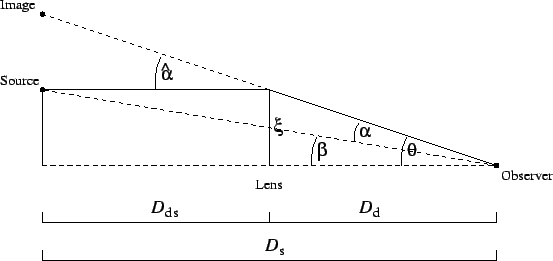
\includegraphics[width=0.7\textwidth]{figures/lens_geometry.png}
	\caption{}
	\label{fig:lens}
\end{figure}

Consider figure \ref{fig:lens}: a ray of light from a source, at a distance $D_s$ from
the observer, deflected due to the lens, at a distance $D_d$ from the observer,  by an 
angle $\hat{\alpha}$ and seen
by the observer at an angle $\theta$ from the lens. If there were no lens, it would have
been observed at $\beta$. Employing small angles approximations, 

\begin{equation}
	\beta  = \theta  - \dfrac{D_{ds}}{D_s} \hat{\alpha}(\xi) \equiv \theta - \alpha(\xi)
	\label{eqn:lens}
\end{equation}
\\
where, $\alpha$ is the scaled deflection angle with respect to the centre of the 
lens to the observed position of the source image and $\xi$ is the impact parameter
of the image on the lens-plane. The equation \ref{eqn:lens} is known
as the {\it lens equation}. The equation describes the true position of the source at $\beta$ to
be seen at $\theta$ due to the lens which is deflecting the light rays by an angle $\alpha$.
If this equation has more than one solution, there will be multiple images of the source. 

For  complex lenses, the 
relation between the deflection angle, $\alpha$, impact parameter, $\xi$ (or $\theta$) and the mass
distribution of the lens can be obtained under the so-called {\it geometrically thin lens}
approximation as,

\begin{equation}
	\alpha(\theta) = \dfrac{1}{\pi} \int d^2\theta^{\prime}
						\kappa(\theta^{\prime})
						\dfrac{\theta-\theta^{\prime}}{|\theta-\theta^{\prime}|^2}
	\label{eqn:alpha}
\end{equation}
\\
where, $\kappa(\theta)$ (or the convergence) is the surface mass density in the 
units of a critical density $\Sigma_{\rm cr}$ defined as,

\begin{equation}
	\kappa(\theta) \equiv \dfrac{\Sigma(\theta)}{\Sigma_{\rm cr}}; 
	\Sigma_{\rm cr} = \dfrac{c^2}{4\pi G} \dfrac{D_s}{D_d D_{ds}}.
\end{equation}

The critical density completely depends on the geometry of the system. For generating
multiple images, $\kappa>1$ and hence the critical density is a characteristic 
surface mass density in order to produce extra images given a source in the background.
Therefore, critical density differentiates between region
of strong and weak lensing, which are described in more details in section \ref{sec:sl}
and \ref{sec:wl}.
\end{comment}


%----------------------------------------------
\subsection{Strong Gravitational Lensing}\label{sec:sl}

Strong gravitational lensing (or SL henceforth), referred to the lensing phenomenon
when the strength of the gravitational field of the lens is sufficiently strong and 
also the alignment between the source, the lens and the observer is optimal enough to
produce multiple images of the source. From equation \ref{eqn:alpha}, SL regime marked
by $\kappa >1$ and relatively small values of $\theta$. So, the multiple images of a
background sources contains information about the projected mass distribution of the lens. 

Given the mass distribution of a lens ($\kappa$) and position of the source ($\beta$),
it is straightforward to find out the position of the multiple images ($\theta$), this process
is called {\it forward modelling}. But given a set of multiple images, which are the main 
observables in SL, it is a highly degenerate process to reconstruct the mass
distribution of the lens. The procedure is referred as {\it lens inversion} or
{\it lens modelling} and mainly consist of reconstructing $\kappa$ and
$\beta$ (as in equation \ref{eqn:timedelay}). 

There are 
several methods for lens inversion. Many of those procedures put strong constraints
on the mass distribution of the lens and assume a functional form and hence are called
as {\it parametric} methods. These methods mainly involve to find the optimal values 
of the free parameters of the functional form of the mass distribution of the lens. 
For example LENSTOOL\footnote{\url{http://projets.lam.fr/projects/lenstool/wiki}} 
\cite{2011ascl.soft02004K}.

There are some methods which invert the lens with minimal assumptions and without
assuming any prior form of the mass distribution of the lens, and are referred as
{\it non-parametric} methods. In these methods, the number of free parameters are often
too large, usually some building block of the total mass maps, and hence larger
statistical consideration is needed. For example, 
Pixelens\footnote{\url{http://www.physik.uzh.ch/~psaha/lens/pixelens.php}} 
\cite{2011ascl.soft02007S}, 
GRALE\footnote{\url{http://research.edm.uhasselt.be/~jori/page/index.php?n=Physics.Grale}}
\cite{2006MNRAS.367.1209L}.

Where parametric models are more efficient, non-parametric models are more
accurate and unbiased. In this work we used a non-parametric lens inversion
library called as GRALE \cite{2006MNRAS.367.1209L,2007MNRAS.380.1729L,2009MNRAS.397..341L} 
to trace the mass distribution of some very massive
galaxy clusters. The building blocks of the mass map are the Plummer spheres, where
other choices such as squares and Gaussian spheres are also available in the library, 
and the total mass map is the super position of these building blocks. GRALE uses
a genetic algorithm (for a review see \citep{1995ApJS..101..309C}) 
to find optimal solution to the weights of the building 
blocks and the resolution of the mass maps is adaptively increased (or decreased)
For more detailed documentation see \cite{2009MNRAS.397..341L}.

Another observable in SL is the time delays between multiple images
of the source. The light rays from the same source travel different directions
and due to the curvature of space time, depending upon the mass distribution 
of the lens, they travel different distances before they reach the same 
observer. Because the distances in cosmology depends on the Hubble constant
or the expansion rate of the Universe, one can calculate the value of the
Hubble constant given measured time delays and mass distribution of the source
\cite{2004tomu.conf..231R}. 
However, it is also possible to have the Hubble constant given and put
additional constraints on the mass distribution of the lens using measured
time delays \cite{2015PASJ...67...21M}.


%----------------------------------------------
\subsection{Weak Gravitational Lensing}\label{sec:wl}

Weak gravitational lensing (or WL henceforth) referred to the phenomenon when 
the lensing is not strong enough to produce multiple images but strong enough
to distort the shape of the source. In WL, deformation matrix is close
to unitary matrix.
The deformation of the shape of the observed galaxies
due to the intervening matter is referred to as {\it cosmic shear}. This
signal is very small, nearly 1-2$\%$ of the intrinsic ellipticity of the source 
and can only be measured statistically under the assumption that the intrinsic 
ellipticity of the background galaxies do not have a preferred direction. If one 
measures the cosmic shear of all background sources behind a lens or mass concentration,
it tends to align tangentially towards the centre of the mass concentration. 

As the signal of the weak lensing cosmic shear is very small as compared to the 
intrinsic ellipticity of the galaxies, this study did not come into play until
the recent observational and technical advancements. Soon 
after the detection of the giant luminous arc in Abell 370, it was observed
that few more objects that are not as stretched as the giant arc but still show
high axis-ratio and are aligned tangentially towards the centre of the cluster. They
termed it as {\it arclets} and it was clear that the alignment is due to the 
gravitational field of the cluster. It was also expected that when there are
only few very strong distortion of the shapes could happen like the giant 
arc, many more smaller distortions can be observed in the background galaxies.
\cite{1990ApJ...349L...1T} reported the first statistical detection of the WL
cosmic shear in two lensing clusters. The theoretical framework was further
formulated by \cite{1993ApJ...404..441K} and it evolved as an active field
to study the mass distribution of lensing clusters in the outskirts. 

Instead of just studying the local mass concentrations, like galaxies or galaxy
clusters, WL can also be used in order to study the statistical distribution of matter
in an inhomogeneous Universe. Light rays coming from all redshift are continuously
distorted from the matter on its path (figure \ref{fig:wl}). 
For example, light from high redshift sources
are deflected many times as they might witness more mass concentrations in its path, 
as compared to low redshift sources. If the cosmic shear can be measured for 
a large ensemble of sources spread over redshift, the statistical properties
of these shears can be used in order to study the statistical properties of the
cosmological matter distribution and hence infer cosmological parameters. The 
theory and its application was first formulated by \cite{1991MNRAS.251..600B}.
One basic requirement of the underlying theory is to give up the geometrically
thin lens approximation and look at the 3D distribution of matter which 
is then projected in 2D sky. The theory of weak lensing and its applications
has been reviewed many times, for a thorough review see: \cite{}.

\begin{figure}
	\centering
	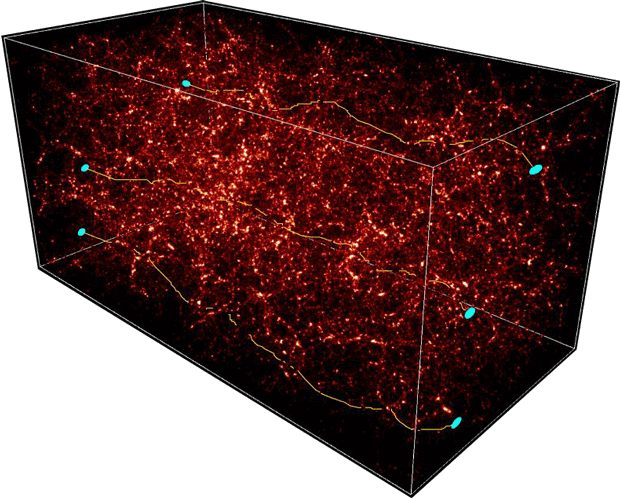
\includegraphics[width=0.7\textwidth]{figures/weaklensing.png}
	\caption{}
	\label{fig:wl}
\end{figure}

Lets first try to model the statistical properties of the convergence field
$\kappa(\theta)$. In cosmological context, the convergence field can be expressed
as the weighted projection of the mass distribution integrated along the line of 
sight,
\begin{equation}
	\kappa(\theta) = \int_0^{\chi_H} g(\chi)\delta(\chi\theta,\chi) \mathrm{d}\chi
\end{equation}
\\
where, $\delta$ is the 3D relative density contrast as defined in the previous section.
$\chi_H$ is the comoving distance to the horizon and $g(\chi)$ is the lensing 
weight. Under the assumption that largest scale structure in $\delta$ are much smaller
than the effective range $\Delta \chi$ of the projection (also known as the Limber's 
approximation), one can write the lensing weights as,

\begin{equation}
	g(\chi) = \dfrac{3H_0^2\Omega_m}{2c^2} \dfrac{\chi}{a(\chi)\bar{n}} \int_{\chi}^{\chi_(H)}
					n(\chi^{\prime})
					\dfrac{(\chi^{\prime}-\chi)}{\chi^{\prime}}\mathrm{d}\chi^{\prime}
\end{equation}
\\
where, $n(\chi)$ gives the distribution of sources as a function of comoving distance or redshift
and $\bar{n}$ is the number of sources per unit area. These quantities depends on the
experiments like Euclid \cite{2013LRR....16....6A}, LSST \cite{2009arXiv0912.0201L} etc.

As mentioned earlier too, the density field $\delta$ is assumed to be a random field
and only its statistical properties can be modelled, not the individual realisations. 
In the previous chapter, we modelled the second order statistics of this random field
as the matter power spectrum, it is interesting to model similar quantity in lensing,
the power spectrum of the convergence field and relate it to the matter power spectrum.


\begin{equation}
	P_{\kappa}(\ell) \equiv \langle |\tilde{\kappa}|^2 \rangle = 
			\int_0^{\chi_H} \dfrac{g(\chi)^2}{\chi^2} 
			P\left(k=\dfrac{\ell}{\chi},\chi \right) d\chi
\end{equation}
\\
where, $\ell = 180/\theta$, is the multipole and give the angle in the sky. 

If the power spectrum of the convergence field $P_{\kappa}(\ell)$ is observable, it can be
used to constrain the 3D matter power spectrum and hence the cosmological parameters. Further,
the same quantity can also be calculated in different redshift bins (instead of just one) and
auto and cross spectra can be obtained. This process is known as 
lensing {\it tomography} and it has extra constraining power over cosmological parameters
\cite{1999ApJ...522L..21H,2004MNRAS.348..897T}.

Now the last problem is to relate the $P_{\kappa}(\ell)$ to something that is observable, 
possibly the cosmic shear. This is rather direct, as in the complex plane Fourier transform
of the comic shear and that of the
convergence can be related with a phase,
\begin{equation}
	\tilde{\gamma(\ell)} = \exp(2i\beta) \tilde{\kappa(\ell)}
\end{equation}
\\
and therefore we have,
\begin{equation}
	\langle |\tilde{\gamma}(\ell)|^2 \rangle = 
	\langle |\tilde{\kappa}(\ell)|^2 \rangle = P_{\kappa}(\ell)
\end{equation}
\\
i.e., the power spectrum of the cosmic shear is the same as the cosmic shear of the
convergence field. Therefore, cosmic shear can be measured in a wide survey and the 
power spectrum is calculated which can be used in order to put constraints on
cosmology.


%----------------------------------------------

%------------------------------------------------------------------------------
%------------------------------------------------------------------------------

\section{Motivation}

The theory of structure formation is partially understood --  at large scales 
or during early dark ages when the perturbations were tiny or only linear order is important. 
However, for small scale clustering processes, when the higher order in perturbations 
become important the analytic solutions are not possible, we rely on simulations and 
approximations. Also, as baryons play a vital role at small scale clustering
and galaxy formation, it is also important to quantify these effects and 
understand various baryonic processes. 
The main motivation of this work is to model the distribution of matter in high dense
regions like lensing clusters and in the large scale structures of the Universe. 
This information is useful in two ways: 

First, the accurate modelling of the matter distribution in individual clusters
give information about the properties of dark-matter. On large scales, dark-matter
is known to be collision-less and non-interacting except for its gravitational effects,
but it is important to quantify and test the hypothesis in high dense regions, like
at the centre of clusters. A small but finite cross section of dark-matter particles
can be well tested in high dense regions, may have stronger implications in our 
understanding of the properties of dark-matter and the Universe in general.  
Also, as the baryonic processes and theory of galaxy
formation is poorly understood, the central regions of the galaxy clusters can be 
used as laboratories to study these processes. It can be done only if the matter 
distribution in the individual systems is well constrained. 
Further, following the hierarchical structure formation, many small haloes interacts and
merge to form large collapsed virialised structures; the study of the distribution of 
matter in lensing clusters at high redshift give information about the merging
stage of the cluster. 

Modelling of the distribution of matter in the large scale structures of the  
Universe is very important
in order to model the cosmological observables. Statistically, the modelling of the
matter power spectrum or 2PCF is important if one wants to do cosmology because 
the matter power spectrum underlies many
cosmological observables like Baryon Accoustic Oscillations (BAO), 
weak lensing, galaxy clustering, redshift
space distortions etc. Also, the modelling of the 
covariance matrix of the matter power spectrum is vital in order to do correct
likelihood analysis and testing cosmological models. Finally baryonic physics 
also changes the power spectrum at small scales, if neglected, it will add biases
in the cosmological parameters and mislead the interpretations. 

\subsection{Challenges}

There are certain challenges in order to accurately model the mass distribution
in clusters and in the Universe. 

\begin{itemize}
	\item Distribution of matter in clusters: Mass is not the observable, what we 
			observe is the light in different frequency bands. We can derive 
			redshift, velocity dispersions etc from this. To relate these observables
			to mass distributions, we have approximations and various models which
			are often rich in systematics, i.e., the incomplete understanding and 
			biases. Gravitational lensing is far the most unbiased technique in order
			to trace matter in lenses. However, even in lensing the inversion of the lens
			is a highly degenerate process. Often and very much in 
			practice, people assume that mass follows light, which is a good approximation
			but may not be true everywhere. So, this is essential that the 
			mass reconstruction techniques are independent of such assumptions in order
			to learn about intrinsic properties of the dark-matter and baryonic
			process in the high dense regions of the lensing clusters.

	\item Modelling matter power spectrum and its covariance matrix: In order to model
			the matter power spectrum at non-linear scales, simulations are far the 
			best solution as all other analytic approaches are difficult. But this is limited
			by the volume and resolution of the simulation. Also a good simulation
			can be very expensive computationally. So, it is possible to simulate a big
			volume at very good resolution for a cosmological realization, but in order
			to carry out a likelihood analysis on some cosmological data, simulations are
			very expensive and impossible to do. So, we rely on semi-analytic models, 
			which can model the matter power spectrum with some function of cosmology
			and are more accurate than the perturbation theories etc at non-linear 
			scales. Similarly, in order to get good covariance matrix of the matter power
			spectrum from simulation, we need to simulate a volume of the order 1000 Gpc/h
			cube, which again is very expensive specially when small scale modelling 
			is necessary. 

	\item Modelling baryonic physics in two-point functions: Finally baryonic effects are 
			important at small scales statistically too. If these effects are not present
			in the model of the power spectrum, it will bias the whole exercise and
			the recovered cosmology might be very precise but not accurate. 
\end{itemize}

So, the main goal of this work is to target these challenges. We perform and completed
a number of projects in order to achieve these goals. 


\subsection{Projects in this work}

In this PhD dissertation, I (along with other collaborators in different projects) tried
to answer few of these question and build a better understanding of distribution of 
matter in the Universe and its clustering properties. 

\begin{itemize}
\item	The very first project is a mass modelling problem in strong lensing cluster
	\cite{2014MNRAS.439.2651M}. Here we
	used a publicly available code GRALE, modified it for an optimum solution and resolution,
	and put tight constraints on the mass distribution of few lensing clusters. By studying
	the mass and light distribution of these clusters, we imply that it is possible 
	that the dark-matter has a finite self-interaction cross section and shows
	important signatures in the central parts of clusters. 

\item	In a similar project, we also show that time delay information is very useful in 
	order to put additional constraints on the central region of the clusters which can't 
	be resolved directly, specially when the steepness degeneracy is broken by the 
	presence of background sources at different redshift \cite{2015PASJ...67...21M}.

\item	We also presented a (semi) analytic model for the matter power spectrum, which is
	computationally inexpensive and compute the power spectrum to a percent level 
	accuracy up to k $\sim$ 1 h/Mpc \cite{2014MNRAS.445.3382M}. 
	The motivation of this model is the halo model
	and we also derived simple form of the covariance matrix. We proposed a way to 
	marginalise over baryonic effects. 

\item	In a similar project to the previous one, we used the halo model in order to directly
	model the effects of baryons on the matter power spectrum and to the extension on the
	weak lensing shear power spectrum \cite{2014arXiv1410.6826M}. 
	The effects are small at comparatively large
	scales but as the next generation surveys are expected to measure these quantities 
	to very small scales, the baryonic effects are important to take into account. If not, 
	it will add biases to the cosmological parameters up to 10 sigma. 

\end{itemize}

\subsection{A unified picture}

If we try to draw a bigger picture from all the projects above, it states that
baryonic physics is very important to model in order to understand the clustering processes,
galaxy formation as well as to do cosmology with future generation surveys. 

Gravitational lensing is one ideal tool to do so. Strong lensing
is very useful in studying the individual systems. 
Weak lensing shear measurements
on larger area in the sky is the most promising tool to do cosmology under
control systematics. One of the biggest source of systematics is again the 
baryonic physics at small scales and there are various ways to handle them. But
they can't be ignored. Precision cosmology and detailed information about the 
individual systems are needed in order to gain full understanding of the 
galaxy formation processes and evolution of the Universe. 






%------------------------------------------------------------------------------







